\section{Results and Figures}\label{sec:figures}
Answer all the parts of the exercise in an organized and clear manner. You should of course try to get good results in all the exercises, but if you have made a good effort without achieving great performance, a good discussion of possible reasons is just as good. Present your thinking and efforts and discuss possible reasons for good or bad results.

Include plots and/or tables of all relevant results, but make sure you don't overwhelm the reader with too many plots. Have a clear plan about what you want to communicate with a specific plot/figure, and use appropriate labels and comments. Keep in mind that the plots should be as ``readable'' as possible; that is, they should not be too hard to interpret and be reasonably self contained.

There are some important things to consider when exporting figures from MATLAB, most importantly which format you use. Never ever use JPEG for anything that is not a photography or similar. Any figure, like a plot or block diagram, must never be stored as a JPEG\@. If you zoom in on \Cref{fig:constraint_jpg} you can see a lot of noise close to any of the dark curves and lines, this is due to the compression in JPEG\@. \Cref{fig:constraint_jpg} will look horrible both on a screen and on paper.

The PNG format is slightly better for plots, but since it is a raster format (a grid of pixels), it looks ugly if you zoom in. It also looks ugly if you scale it, both on a screen and on paper. Try to avoid PNG if you can. \Cref{fig:constraint_png,fig:constraint_png_large} are both PNG figures; the latter being a larger figure scaled more than the former. Note both how choppy and ugly the blue curve is, and how the different sizes create inconsistent font sizes.

The simplest way to get a reasonably good looking plot is to save it as EPS in MATLAB\@. Do this by clicking ``File'' in the figure window, and the ``Save As\ldots''; choose ``EPS file (*.eps)'' in the ``Save as type:'' menu.\footnote{pdfLatex does not support EPS directly, but since we have loaded the \emph{epstodf} package, this is not a problem.} \Cref{fig:constraint_eps} shows a plot in EPS format. Since EPS is a vector format, the Figure can be scaled and still look good (but mind the font size!). If you zoom in you can see that the curve and the letters/numbers are smooth. A figure in vector format will usually look good both on a screen and on paper.

Note that the size of the actual figure window in MATLAB determines how large the exported figure is. Hence, if you enlarge the figure window before exporting, you will need to scale the figure by a larger factor in the report. This will lead to a tiny font in the figure. There are many better ways of exporting graphics from MATLAB, but they quickly become fairly involved. The above method of exporting to EPS will in most cases give nice figures.

You can write Latex in your MATLAB figures. The script used to create \Cref{fig:constraint_jpg,fig:constraint_eps} is included in \Cref{sec:plot_constraint_m}. Do not use a screen shot of a scope of figure in MATLAB in your report.

\begin{figure}[htb]
	\centering
		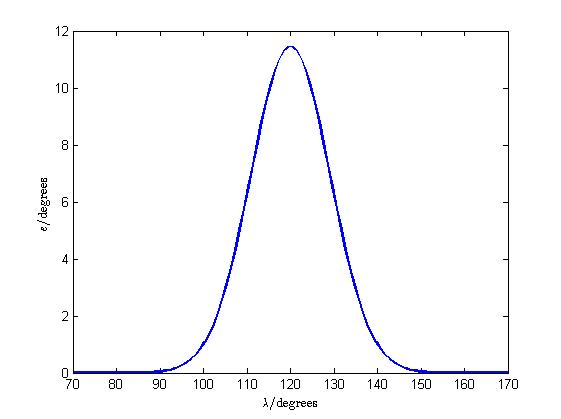
\includegraphics[width=0.8\textwidth]{figures/template/constraint_jpg.jpg}
	\caption{A plot in JPEG format --- a very bad idea.}
\label{fig:constraint_jpg}
\end{figure}

\begin{figure}[htb]
	\centering
		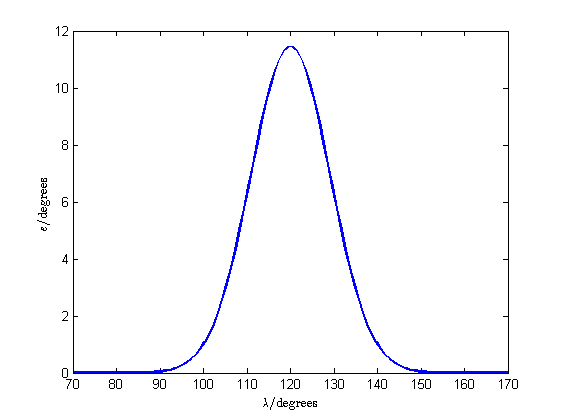
\includegraphics[width=0.8\textwidth]{figures/template/constraint_png.png}
	\caption{A plot in PNG format --- a bad idea.}
\label{fig:constraint_png}
\end{figure}

\begin{figure}[htb]
	\centering
		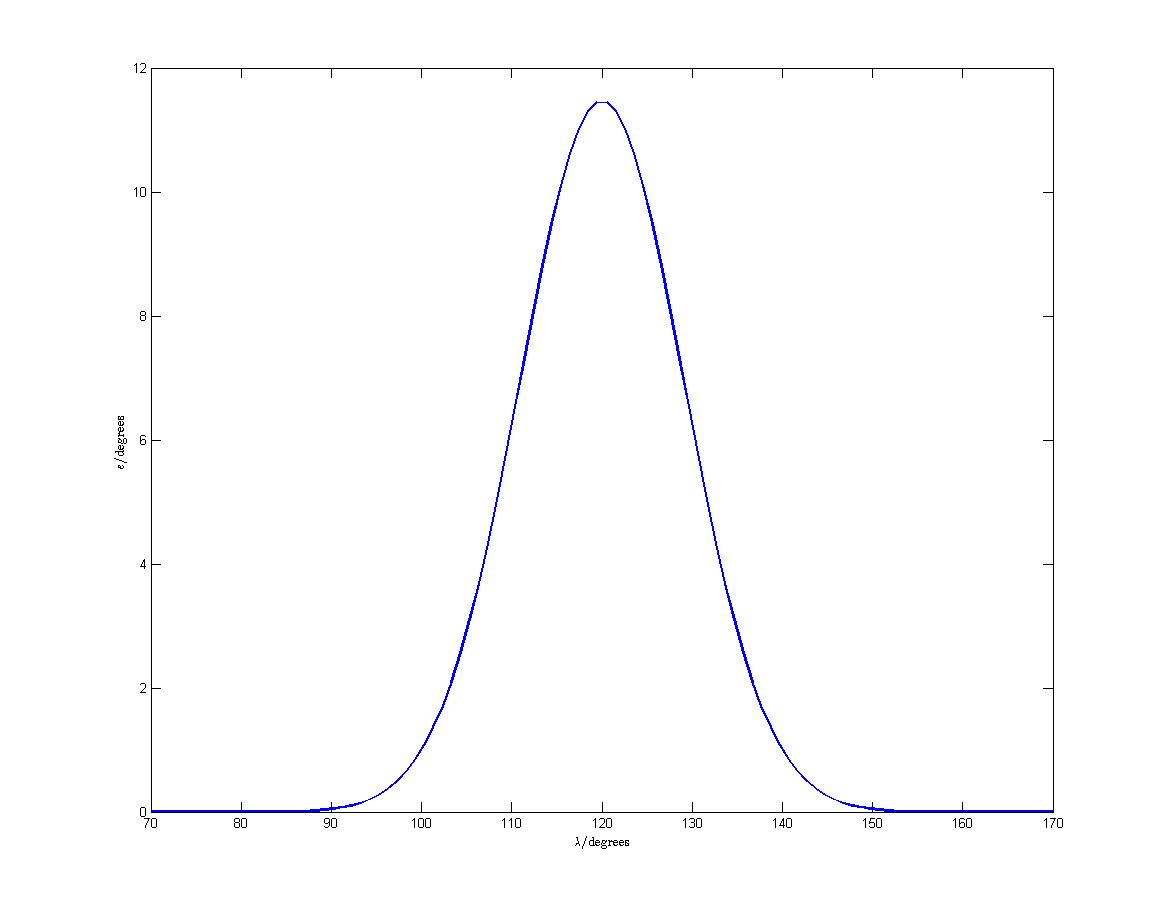
\includegraphics[width=0.8\textwidth]{figures/template/constraint_png_large.png}
	\caption{A plot in PNG format --- a bad idea. This figure is originally larger than the other PNG figure, but both are scaled to the same size.}
\label{fig:constraint_png_large}
\end{figure}

\begin{figure}[htb]
	\centering
		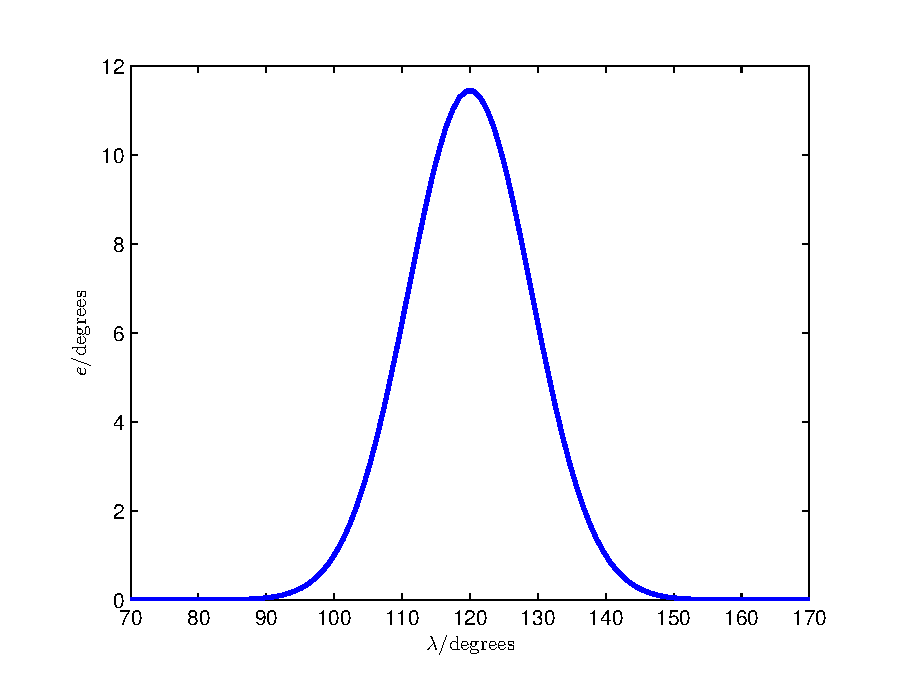
\includegraphics[width=0.8\textwidth]{figures/template/constraint_eps.eps}
	\caption{A plot in EPS format --- a much better idea.}
\label{fig:constraint_eps}
\end{figure}

Remember to reference all figures in the text. Figures have a number and should be referenced by that number (again, always use dynamic references). They also tend to float around, meaning they generally don't appear where you ask them to in the text. This is fine, do not try to force a figure (or a table) to appear in a particular place. As long a you refer to it, it's easy to find. No figure should be included without being referenced in the text.

If you look at the source code for including figures, you can see that the optional option \verb+[htb]+ has been used. This tells Latex where you wish the figure to appear, in prioritized order. \verb+h+ means ``Here'', t means ``Top of this page'', b means ``Bottom of this page'', and p (not used here) means ``on a Page with only floats (such as figures and tables)''. Note that your wish might not be granted, and this is because Latex actually optimizes the placement of figures. If you start forcing figures to be in specific places, it often leads to really strange layout somewhere else in the document. 

Generally, let Latex handle the documentation layout. This is one of the main reasons to choose Latex over software such as Microsoft Word.

\subsection{Results and Discussion}
All problems should have their own discussion of results. 

Remember: all plots and results need a description, explanation, and discussion.
